% Template for Elsevier CRC journal article
% version 1.2 dated 09 May 2011

% This file (c) 2009-2011 Elsevier Ltd.  Modifications may be freely made,
% provided the edited file is saved under a different name

% This file contains modifications for Procedia Computer Science

% Changes since version 1.1
% - added "procedia" option compliant with ecrc.sty version 1.2a
%   (makes the layout approximately the same as the Word CRC template)
% - added example for generating copyright line in abstract

%-----------------------------------------------------------------------------------

%% This template uses the elsarticle.cls document class and the extension package ecrc.sty
%% For full documentation on usage of elsarticle.cls, consult the documentation "elsdoc.pdf"
%% Further resources available at http://www.elsevier.com/latex

%-----------------------------------------------------------------------------------

%%%%%%%%%%%%%%%%%%%%%%%%%%%%%%%%%%%%%%%%%%%%%%%%%%%%%%%%%%%%%%
%%%%%%%%%%%%%%%%%%%%%%%%%%%%%%%%%%%%%%%%%%%%%%%%%%%%%%%%%%%%%%
%%                                                          %%
%% Important note on usage                                  %%
%% -----------------------                                  %%
%% This file should normally be compiled with PDFLaTeX      %%
%% Using standard LaTeX should work but may produce clashes %%
%%                                                          %%
%%%%%%%%%%%%%%%%%%%%%%%%%%%%%%%%%%%%%%%%%%%%%%%%%%%%%%%%%%%%%%
%%%%%%%%%%%%%%%%%%%%%%%%%%%%%%%%%%%%%%%%%%%%%%%%%%%%%%%%%%%%%%

%% The '3p' and 'times' class options of elsarticle are used for Elsevier CRC
%% The 'procedia' option causes ecrc to approximate to the Word template
\documentclass[3p,times,procedia]{elsarticle}
\flushbottom

%% The `ecrc' package must be called to make the CRC functionality available
\usepackage{ecrc}
\usepackage[bookmarks=false]{hyperref}
    \hypersetup{colorlinks,
      linkcolor=blue,
      citecolor=blue,
      urlcolor=blue}
%\usepackage{amsmath}

\usepackage{wrapfig}
\usepackage{graphicx}
\usepackage[export]{adjustbox}

%% The ecrc package defines commands needed for running heads and logos.
%% For running heads, you can set the journal name, the volume, the starting page and the authors

%% set the volume if you know. Otherwise `00'
\volume{00}

%% set the starting page if not 1
\firstpage{1}

%% Give the name of the journal
\journalname{Procedia Computer Science}

%% Give the author list to appear in the running head
\runauth{William Charlton}

%% The choice of journal logo is determined by the \jid and \jnltitlelogo commands.
%% A user-supplied logo with the name <\jid>logo.pdf will be inserted if present.
%% e.g. if \jid{yspmi} the system will look for a file yspmilogo.pdf
%% Otherwise the content of \jnltitlelogo will be set between horizontal lines as a default logo

%% Give the abbreviation of the Journal.
\jid{procs}

%% Give a short journal name for the dummy logo (if needed)
%\jnltitlelogo{Computer Science}

%% Hereafter the template follows `elsarticle'.
%% For more details see the existing template files elsarticle-template-harv.tex and elsarticle-template-num.tex.

%% Elsevier CRC generally uses a numbered reference style
%% For this, the conventions of elsarticle-template-num.tex should be followed (included below)
%% If using BibTeX, use the style file elsarticle-num.bst

%% End of ecrc-specific commands
%%%%%%%%%%%%%%%%%%%%%%%%%%%%%%%%%%%%%%%%%%%%%%%%%%%%%%%%%%%%%%%%%%%%%%%%%%

%% The amssymb package provides various useful mathematical symbols

\usepackage{amssymb}
%% The amsthm package provides extended theorem environments
%% \usepackage{amsthm}

%% The lineno packages adds line numbers. Start line numbering with
%% \begin{linenumbers}, end it with \end{linenumbers}. Or switch it on
%% for the whole article with \linenumbers after \end{frontmatter}.
%% \usepackage{lineno}

%% natbib.sty is loaded by default. However, natbib options can be
%% provided with \biboptions{...} command. Following options are
%% valid:

%%   round  -  round parentheses are used (default)
%%   square -  square brackets are used   [option]
%%   curly  -  curly braces are used      {option}
%%   angle  -  angle brackets are used    <option>
%%   semicolon  -  multiple citations separated by semi-colon
%%   colon  - same as semicolon, an earlier confusion
%%   comma  -  separated by comma
%%   numbers-  selects numerical citations
%%   super  -  numerical citations as superscripts
%%   sort   -  sorts multiple citations according to order in ref. list
%%   sort&compress   -  like sort, but also compresses numerical citations
%%   compress - compresses without sorting
%%
%% \biboptions{authoryear}

% \biboptions{}

% if you have landscape tables
\usepackage[figuresright]{rotating}
%\usepackage{harvard}
% put your own definitions here:x
%   \newcommand{\cZ}{\cal{Z}}
%   \newtheorem{def}{Definition}[section]
%   ...

% add words to TeX's hyphenation exception list
%\hyphenation{author another created financial paper re-commend-ed Post-Script}

% declarations for front matter

\begin{document}
\begin{frontmatter}

%% Title, authors and addresses

%% use the tnoteref command within \title for footnotes;
%% use the tnotetext command for the associated footnote;
%% use the fnref command within \author or \address for footnotes;
%% use the fntext command for the associated footnote;
%% use the corref command within \author for corresponding author footnotes;
%% use the cortext command for the associated footnote;
%% use the ead command for the email address,
%% and the form \ead[url] for the home page:
%%
%% \title{Title\tnoteref{label1}}
%% \tnotetext[label1]{}
%% \author{Name\corref{cor1}\fnref{label2}}
%% \ead{email address}
%% \ead[url]{home page}
%% \fntext[label2]{}
%% \cortext[cor1]{}
%% \address{Address\fnref{label3}}
%% \fntext[label3]{}

\dochead{The 12th International Workshop on Agent-based Mobility, Traffic and Transportation Models, Methodologies and Applications (ABMTrans 2023)\\ March 15-17, 2023, Leuven, Belgium}%
%% Use \dochead if there is an article header, e.g. \dochead{Short communication}
%% \dochead can also be used to include a conference title, if directed by the editors
%% e.g. \dochead{17th International Conference on Dynamical Processes in Excited States of Solids}

\title{SimWrapper, an open source web-based platform for interactive visualization of microsimulation outputs and transport data}

\author[a]{William Charlton*}
\author[b]{Bhargava Sana}

\address[a]{Technische Universität Berlin, Chair of Transport Systems Planning and Transport Telematics, Straße des 17. Juni 135, 10623 Berlin, Germany}
\address[b]{San Diego Association of Governments, 401 B Street, Unit 800, San Diego, CA 92101, United States}

\begin{abstract}
A new open-source, web-based, configurable data visualization platform is presented that is specifically designed to support large-scale transportation simulations including MATSim and ActivitySim. It produces a wide array of interactive charts, maps, animations and analysis dashboards that are generally useful in the transportation domain. Interactive visualizations can be created and viewed locally on an analyst's laptop, or public web-based dashboards can be published for viewing on the open Internet. The details of software design are provided along with several examples of implementation at public agencies. User feedback shows the platform is found to be very flexible, while the straightforward configuration approach enables efficient development and deployment of web-based interactive visualizations. While it is not intended to replace geographic information systems or commercial software packages, the smaller curated set of capabilities is found by users to warrant its current adoption at several public agencies. Further work is needed to add more useful features, improve the platform's quality and user experience, and extend documentation.

\end{abstract}

\begin{keyword}
Data visualization; Data dashboards; Transport microsimulation; Human-Computer Interaction; MATSim; ActivitySim
\end{keyword}
\cortext[cor1]{Corresponding author. Tel.: +1-415-335-9282}
\end{frontmatter}

\email{charlton@vsp.tu-berlin.de}

%% main text
%\enlargethispage{-7mm}

%% ###########################################################################

\section{Introduction}

Data visualization has been an integral part of transportation planning and travel forecasting for decades \cite{dueker1990geographic}. More recently, transportation data visualizations have become interactive and can also be shared over the web \cite{NAP24755}. This paper describes SimWrapper, an advanced data visualization platform that is unique because it is open source, web-based, specifically targets transportation simulation and activity-based model outputs, is actively developed, and is already in use in several locations worldwide.

SimWrapper was originally developed by the Transport Planning and Telematics department at Technische Universität Berlin (TU Berlin) to support MATSim, an agent-based microsimulation framework for large-scale transportation simulations \cite{MATSimBook}. TU Berlin has been researching open source, web-based visualization platforms for displaying MATSim results since 2017.  These tools have taken various names including MatHub \cite{CharltonLaudan2020WebBasedVisualization} and AfterSim \cite{CHARLTON2021728}, and SimWrapper is the latest iteration of this research with some interesting and unique capabilities.

The platform produces a wide array of interactive charts, maps, and dashboards that are generally useful in the transportation domain. User feedback shows the platform is found to be flexible, and straightforward configuration using text files enables efficient development and deployment of repeatable and deployable web-based interactive visualizations. The details of software design are provided below along with some examples of implementation at public agencies.

This new platform, SimWrapper, in a nutshell:

\begin{itemize}[]
\item
    is a static website in the form of a ``single page application'' that is compatible with all modern web browsers;
\item
    allows the user to navigate their local filesystem folders in-browser, rather than uploading files to a central server or database. This matches the design of MATSim and other simulation frameworks which all produce collections of output files by default;
\item
    also supports network-based file storage for public- and/or group-accessible shared data (such as model runs or simulation outputs), for internal collaboration and for world-accessible project dashboards;
\item
    provides a collection of data visualization archetypes, e.g. statistical charts, geographic data viewers supporting road and transit network link data, area aggregation maps, X/Y coordinate plots, agent animations, and more;
\item
    can combine all of these components into cohesive dashboards that the user can lay out in a flexible manner, using drag and drop or by editing small text files. These configurations can be applied project-wide;
\item
    enables easy and cost-free online publishing of results.
\end{itemize}

SimWrapper can be deployed on a local network or accessed directly from the main SimWrapper website linked at the end of this paper. It is used by several project teams at TU Berlin and by some public agencies. SimWrapper is generic enough to be broadly useful, but it is not intended to replace GIS tools nor commercial analysis packages.

% ============================================================
\section{State of research}

Numerious past studies present visualization tools and platforms that were developed to cater to the needs of a broad range of applications, ranging from visualizing traffic microsimulation \cite{CHARLTON2021728,lu2015global}, and transportation accessibility \cite{yin2015understanding} to highway performance measures \cite{NAP26651}.

Previous literature reveals that the number of web-based interactive platforms specifically developed for visualizing travel demand model inputs and outputs is still limited. Agent-based microsimulation and activity-based models are gaining popularity in recent years due to higher policy sensitivity and behavioral realism \cite{LempMcWethy2007}, and with them the input and output datasets are increasing in granularity and complexity.

Consequently, there is a growing need for tools that can effectively visualize these datasets. The visualizations could potentially be used for a variety of purposes such as conducting quality checks on model inputs, summarizing simulation outputs, comparing outputs across different scenarios, etc. In addition, they may be needed to communicate the findings of travel modeling efforts and analyses to decision-makers and the public, who are less and less interested in reading PDF reports \cite{KAHILATANI201945}.

% ============================================================
\section{SimWrapper: design and implementation}

SimWrapper is an open source and web-based data visualization platform intended for researchers who wish to build interactive dashboards that display the results of their simulations and model runs. The platform is designed as a standalone website which is configured to access files stored on the local machine, on network file servers, or using internet-based file storage.

Initial internal discussions identified necessary capabilities which were then augmented through iterative trial and error fashion. Like many other dashboard tools, SimWrapper can display interactive charts such as bar, line, pie, and scatterplots. But SimWrapper can also create many advanced map-based visualizations of large disaggregate datasets derived from MATSim and ActivitySim \cite{ActivitySim}, described below. Each of these can be viewed individually or combined into cohesive dashboards.

The high-level workflow is as follows: after running a simulation, some outputs such as MATSim trips and events can be directly viewed in SimWrapper, while other outputs require some post-processing to produce summary datasets in comma-separated value (CSV) format. Along with the data, the user provides configuration details for each dashboard which define the layout and any additional parameters. Typical configuration details are the names and locations of input files, color and width symbology specifications, and so on. These parameters can be set on a project level or for individual runs, and are stored as specially-formatted text files using the common "YAML" text markup format. The website reads these files and generates the dashboards. Dashboards can be organized as separate pages, be full-screen, or use a special side-by-side mode for comparison tasks.

End users are not expected to know or use JavaScript, Python or any other notebook programming language; SimWrapper is essentially just a website like any other. It reads the files directly and builds visualizations according to the text configuration files in those same folders.

\subsection{User feedback on the design approach}

Previous research showed that most regular users in the middle of their research workflow run simulations either on their personal laptop/desktop machines, or on shared compute cluster machines with large storage but no public-facing access to the web. These runs are usually not intended to be immediately published. Analysts often run and review scenarios on their local machines, and then publish “good” runs to a departmental file server.

User feedback from early versions of the tool made two design goals clear: (1) analysts do not want to duplicate and upload their large output files to a new system, and (2) building consistent visualizations across model runs requires the configuration details to be copyable amongst runs.

The first design goal requires finding a way to grant the user's web browser access to select folders on their local filesystem. With Google Chrome and Microsoft Edge, this is as simple as clicking “yes” to a security popup when using the site. For other browsers, a small companion program (link at the end) is provided which runs in the user's top-level data folder. This tool runs a local web (HTTP) server that grants the needed access to files and folders in its startup folder.

The second goal, creating consistent visualizations, is accomplished by authoring configuration files which can be shared among runs or copied between folders as needed. Initially, visualizations can can be created interactively using the website, choosing details such as datasets, colors, scales, etc. Then an export button writes the configuration to a text file which can be copied or modified as needed.

This provides a \textit{``best of both worlds''} design where the user isn't expected to memorize the configuration file format and can produce valid configurations using the website itself; but they can also edit the exported text file to rapidly make small changes and share them across model runs.

\subsection{Managing, accessing, and publishing files with SimWrapper}

Eventually, most users of SimWrapper wish to publish their dashboards (either internally or on the web), so a method for accessing network-based file resources is also provided. For this, the server needs to provide HTTP-based file and folder browsing via a defined URL. This is easily configured on any web server such as NGINX or Apache, and every cloud-based service also provides this option. The configuration details are provided on the SimWrapper website.

The public TU Berlin file server is one such data source, but others can be added by end users. Each source must allow HTTP-based directory access to this storage: SimWrapper needs to be able to \emph{view directory listings} and \emph{retrieve file contents}. SimWrapper never writes any files anywhere itself; it is a read-only system.

To actually publish a SimWrapper-based website online, one simply clones or copies the website code from the SimWrapper website, copies all data and configuration files to the \textit{data} subfolder, and pushes it to any static web host, such as GitHub Pages. More details are on the SimWrapper website.

% For more examples, reference the primary TU Berlin SimWrapper website which hosts a gallery of many example dashboards on its public file server.

% \subsubsection{Data security and privacy}

% The SimWrapper site itself is loaded from the Internet, but once loaded, the user's data never leaves their computer. SimWrapper is an entirely client-side system with absolutely no upstream data server. Data is loaded into the browser from wherever, but nothing leaves the browser. The SimWrapper website is fully open source, collects no user information, stores no cookies, never sees user data, and therefore has minimal privacy implications.

%% ======================================================================
%% ======================================================================
%% ======================================================================
\section{Some key and noteworthy data visualizations implemented in SimWrapper}

Figures 1 and 2 show example dashboards with sample data, to give the reader an idea of what is possible with SimWrapper. Unfortunately, the human-computer interface of an interactive plot is impossible to capture in a PDF.

The \textbf{link viewer} can display networks in MATSim or shapefile formats. Datasets can be joined by link ID, and then symbology and filtering is configured in the UI or via YAML configuration.

An \textbf{area map} visualization allows shapefiles and area-based maps to be created with line, color, fill, filter, and difference symbologies. Multiple datasets can be joined to the area boundaries and maps can be interactively developed and then exported to YAML.

\textbf{X/Y points and X/Y hexagon} viewers handle point data, as not all transport data is link-based. Activity locations, home locations, pickups and dropoffs for transit and taxi modes, all have geographic coordinates associated with them. For this type of point data, two visualizations are provided: one which displays point data directly, possibly linked to time-of-day, and the other which aggregates point data into equal-size hexagons across the map. The default MATSim file \textit{output\_trips.csv} is automatically viewable using this visualization.

\begin{figure}
  \centering
  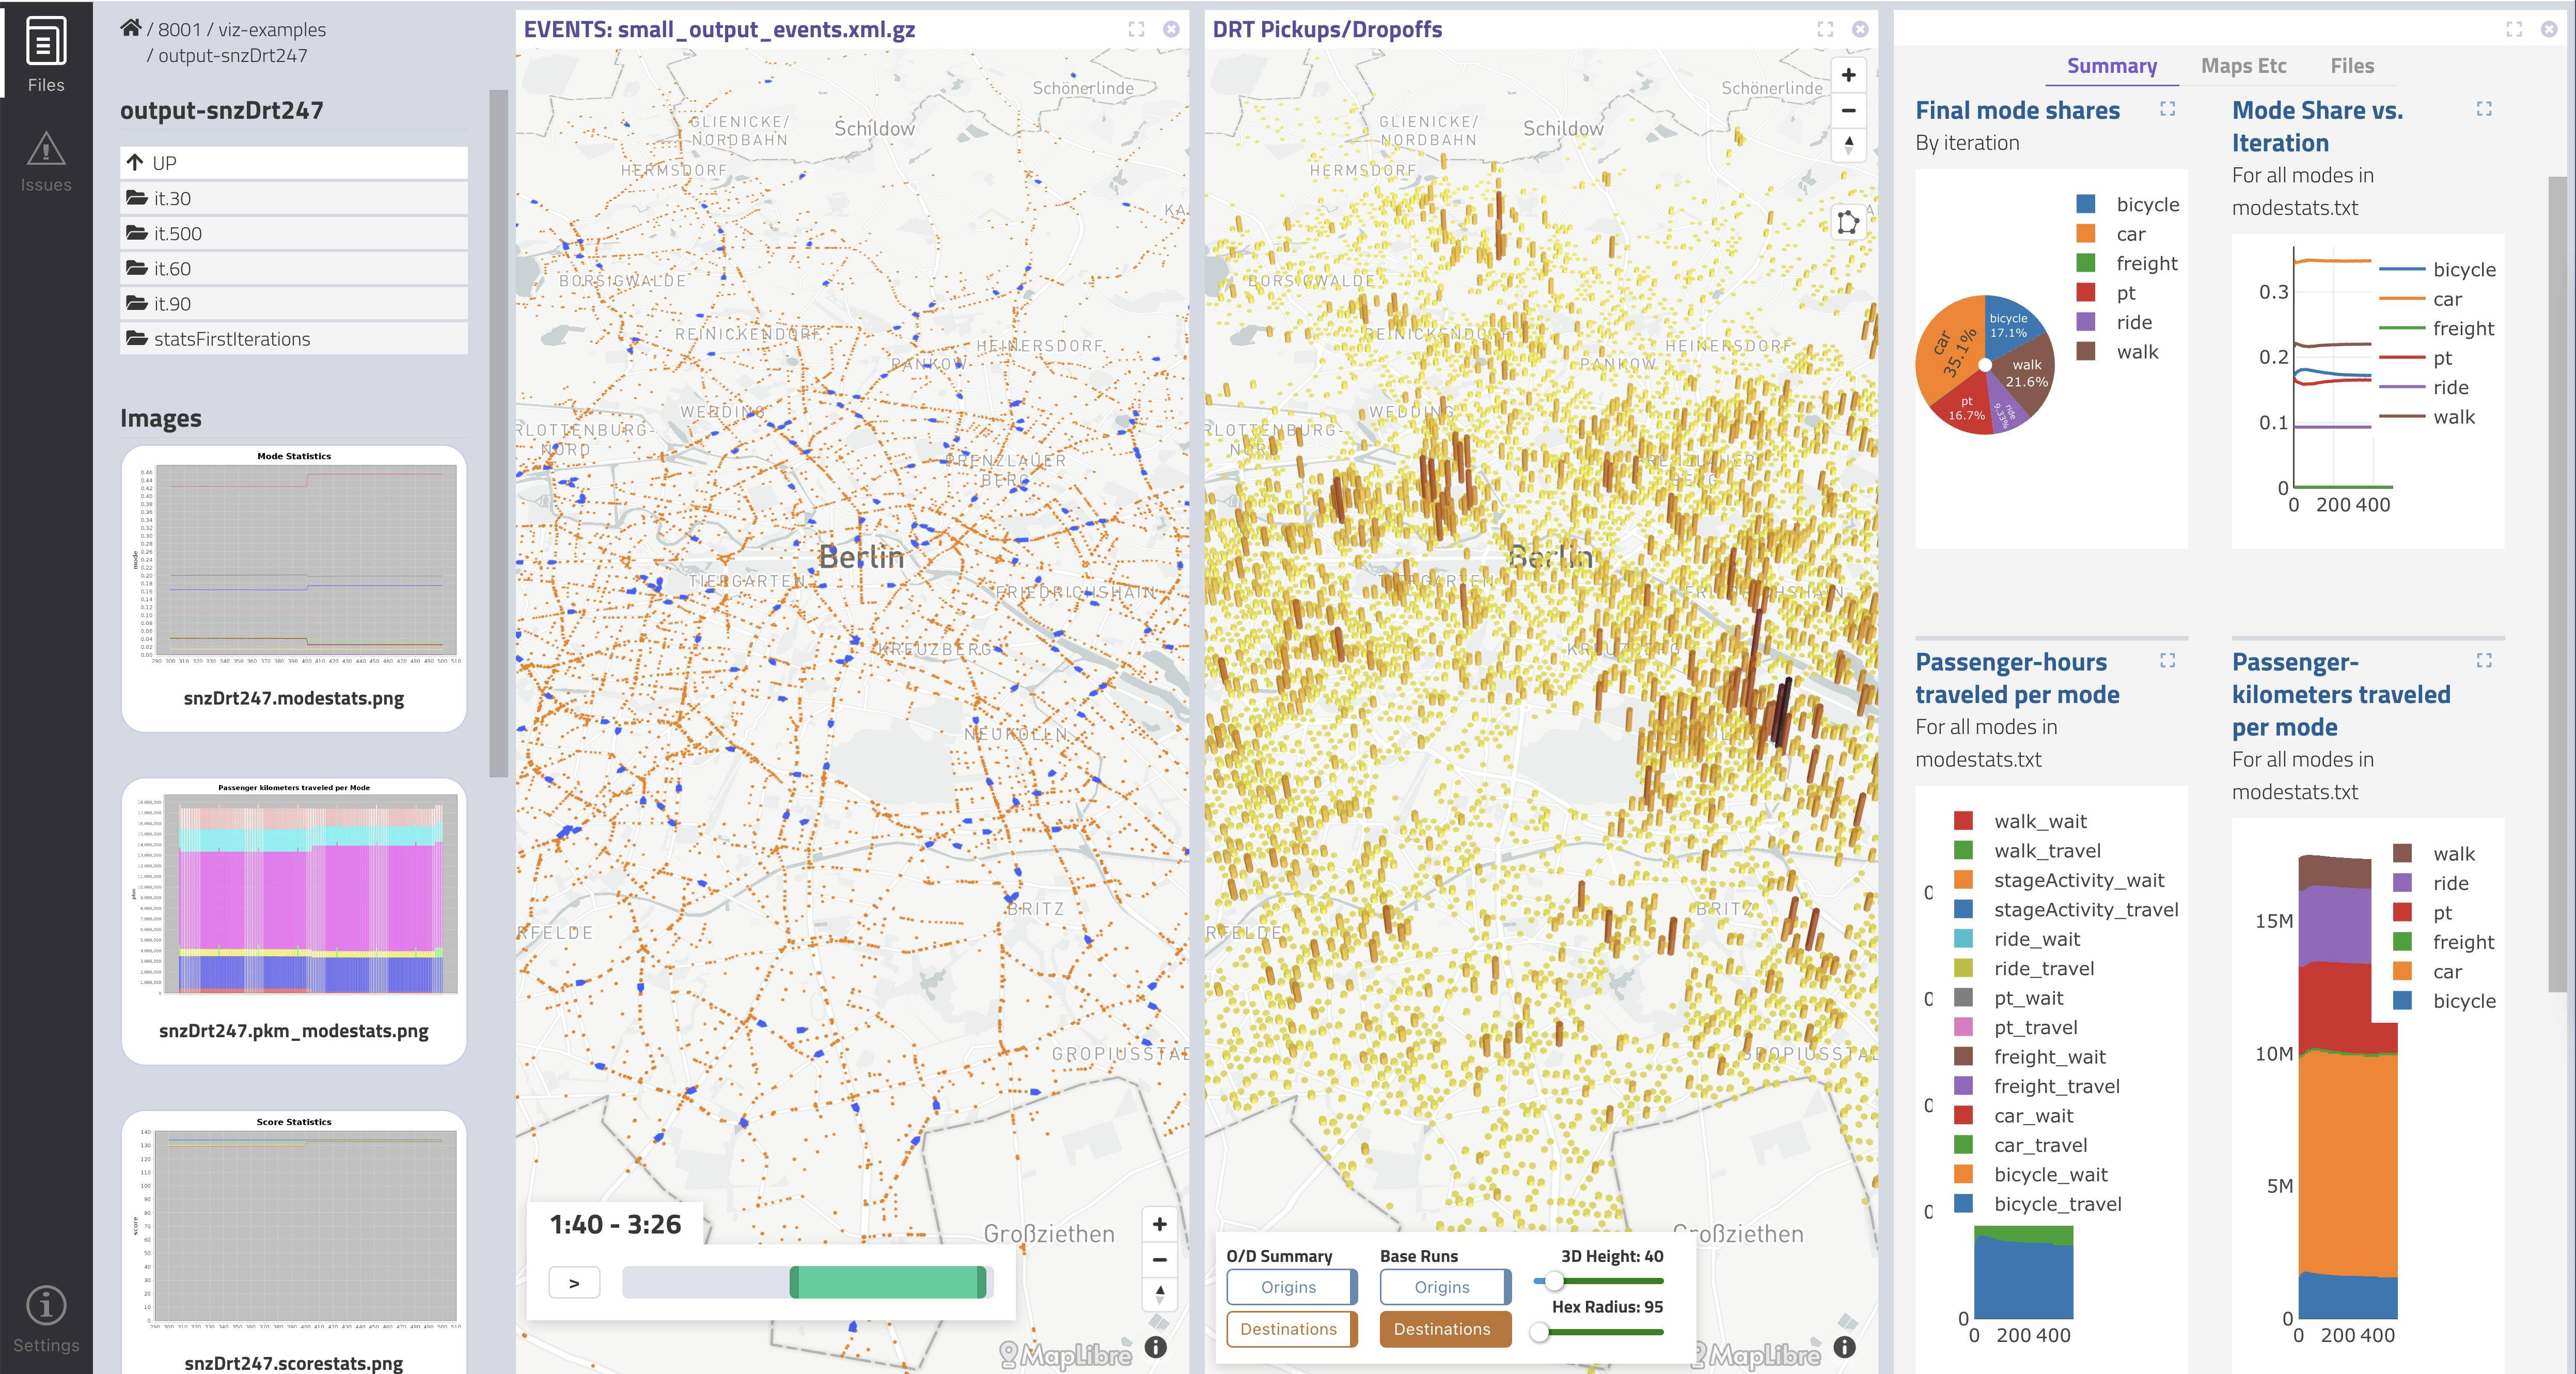
\includegraphics[width=\textwidth,height=2.8in]{images/fig-dashboard-1.jpg}
  \caption{Example dashboard showing (a) vehicle animation and point data, (b) point data aggregated into areas; (c) some basic chart summaries}
  \label{fig:chart1}
\end{figure}

A \textbf{vehicle animation} for MATSim event files allows interactive viewing of vehicle trajectories on a second-by-second basis. Postprocessing can enable the user to focus on specific markets or modes such as autonomous vehicle fleets.

Left out due to space considerations are the basic charts, Vega-Lite\cite{VegaLiteWebsite}  advanced charts; MATSim transit networks; MATSim freight/carriers; aggregate origin/destination plots; and a summary table / calculation generator.

\begin{figure}
  \centering
  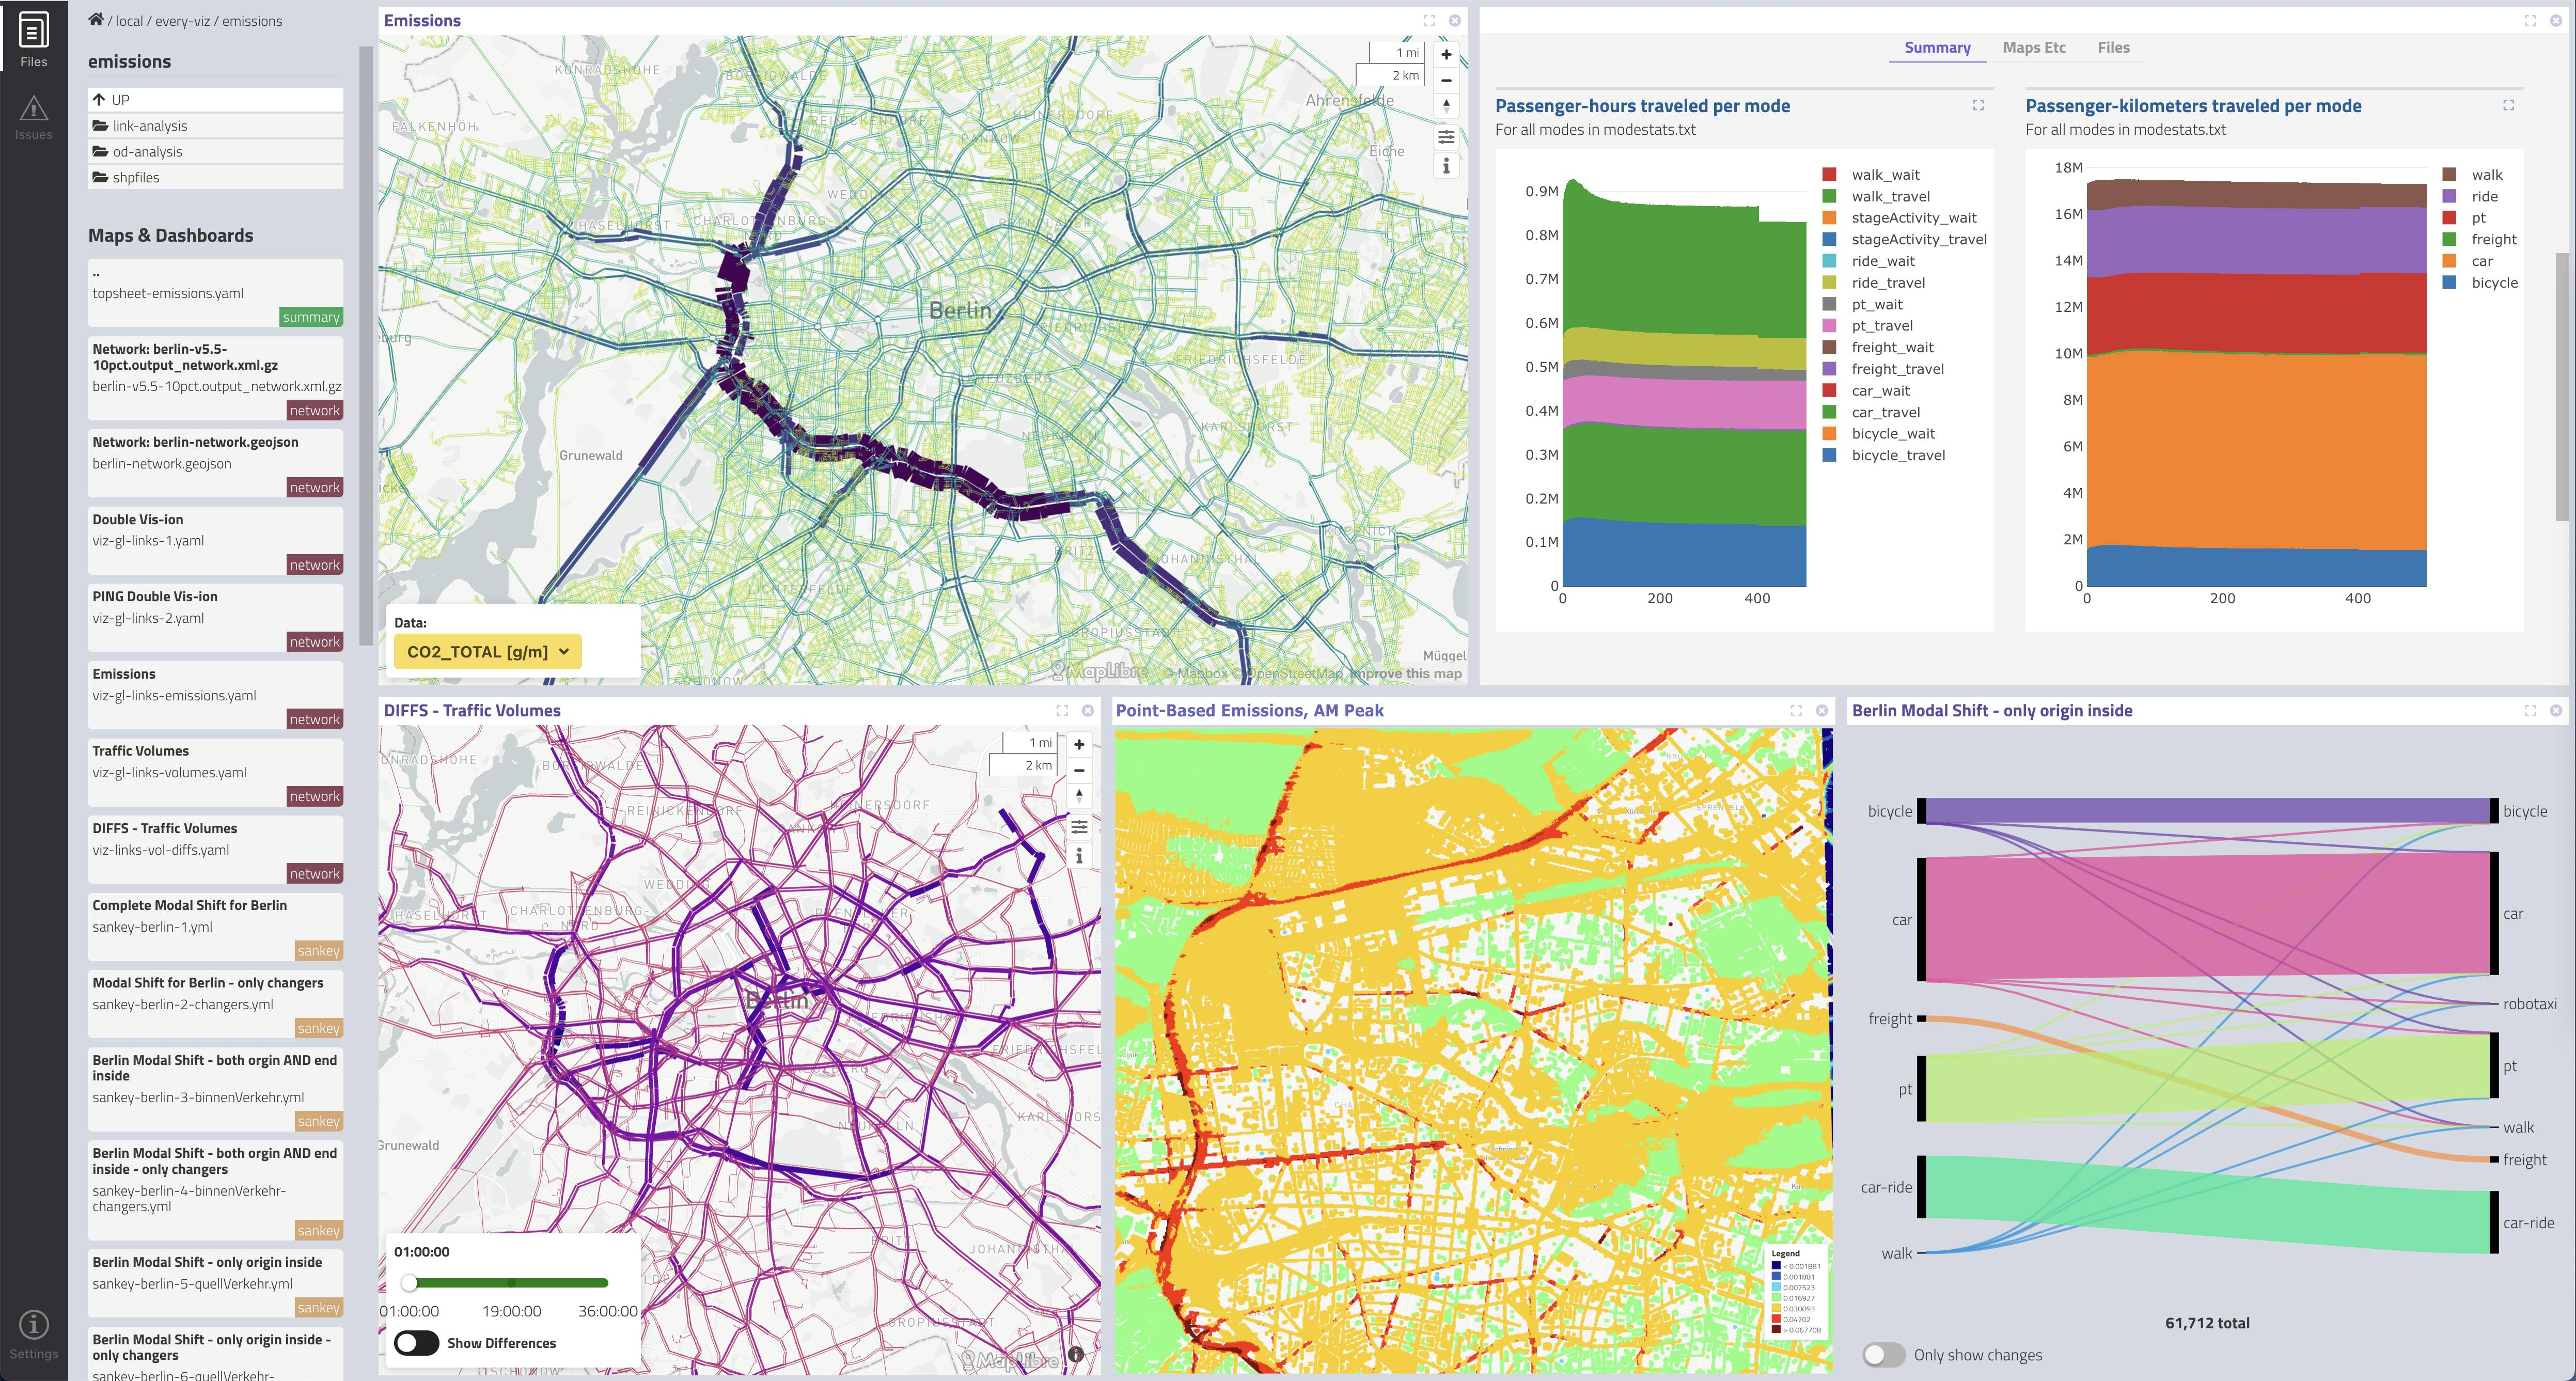
\includegraphics[width=\textwidth,height=3in]{images/fig-dashboard-2.jpg}
  \caption{Example dashboard depicting network link, X/Y point-based emissions, and mode shift diagrams}
  \label{fig:chart2}
\end{figure}



% --------------------------------------------------------------------
% \subsection{Summary calculations: providing top-line summary metrics}

% --------------------------------------------------------------------
% \subsection{Summary calculations: providing top-line summary metrics}

% Top-level summaries provide the first indication of useful or erroneous results, such as overall mode share, average travel times, total emissions, and so forth. These measures are an excellent way to "sanity-check" a model run; in other words, to identify any suspect results or errors when compared to previously-established norms.

% The most robust way to generate and display a complex calculation is to create a custom post-processing script tailored to the job, which outputs a simple CSV with the needed values. Especially for more complex post-processing needs, using a high-quality platform such as Python or R is the recommended path.

% For more simple summaries, we developed a way to extract and minimally process typical CSV and XML data file formats. This is based on experience with the hesitancy of some analysts in our department to write Python and R scripts. A special YAML configuration schema for calculations has four sections: \textbf{files}, the set of CSV or XML input files;  \textbf{interactive inputs}, entries in the UI where users can provide values directly (imagine fuel cost per liter, or number of vehicles in a taxi fleet); \textbf{calculations}, an ordered list of mathematical variables and equations, based on the data columns and inputs in the previous sections; finally, \textbf{outputs}, the entries to be displayed in the dashboard.

% The details of the calculation engine domain-specific language (DSL) specification are available on the main SimWrapper documentation website.


%% ======================================================================
%% ======================================================================
%% ======================================================================
\section{Example projects using SimWrapper}

%% ======================================================================
\textbf{KoMo:Dnext (Düsseldorf, Germany)}: An extensive dashboard for the MATSim Düsseldorf transport scenarios, including link flow capacities and volumes, statistical charts, videos, and more. Figure 3 shows a small portion of the site. Viewable online at \textit{vsp.berlin/simwrapper/komodnext}

\textbf{SF-CHAMP: San Francisco, California, USA}. SF-CHAMP is the activity-based model used by the San Francisco County Transportation Authority (SFCTA)\cite{outwater2006san}. SFCTA uses SimWrapper to perform quality control on model inputs and to review model outputs, using both the area map and the link viewer.

There is no room for screenshots of the SF-CHAMP project sites, nor is there room for showcasing other projects using SimWrapper, including the ActivitySim consortium of agencies using it in the United States, and the excellent dashboard for the RealLabHH project in Hamburg, Germany, available online for review at \textit{vsp.berlin/simwrapper}.

\begin{figure}
  \centering
  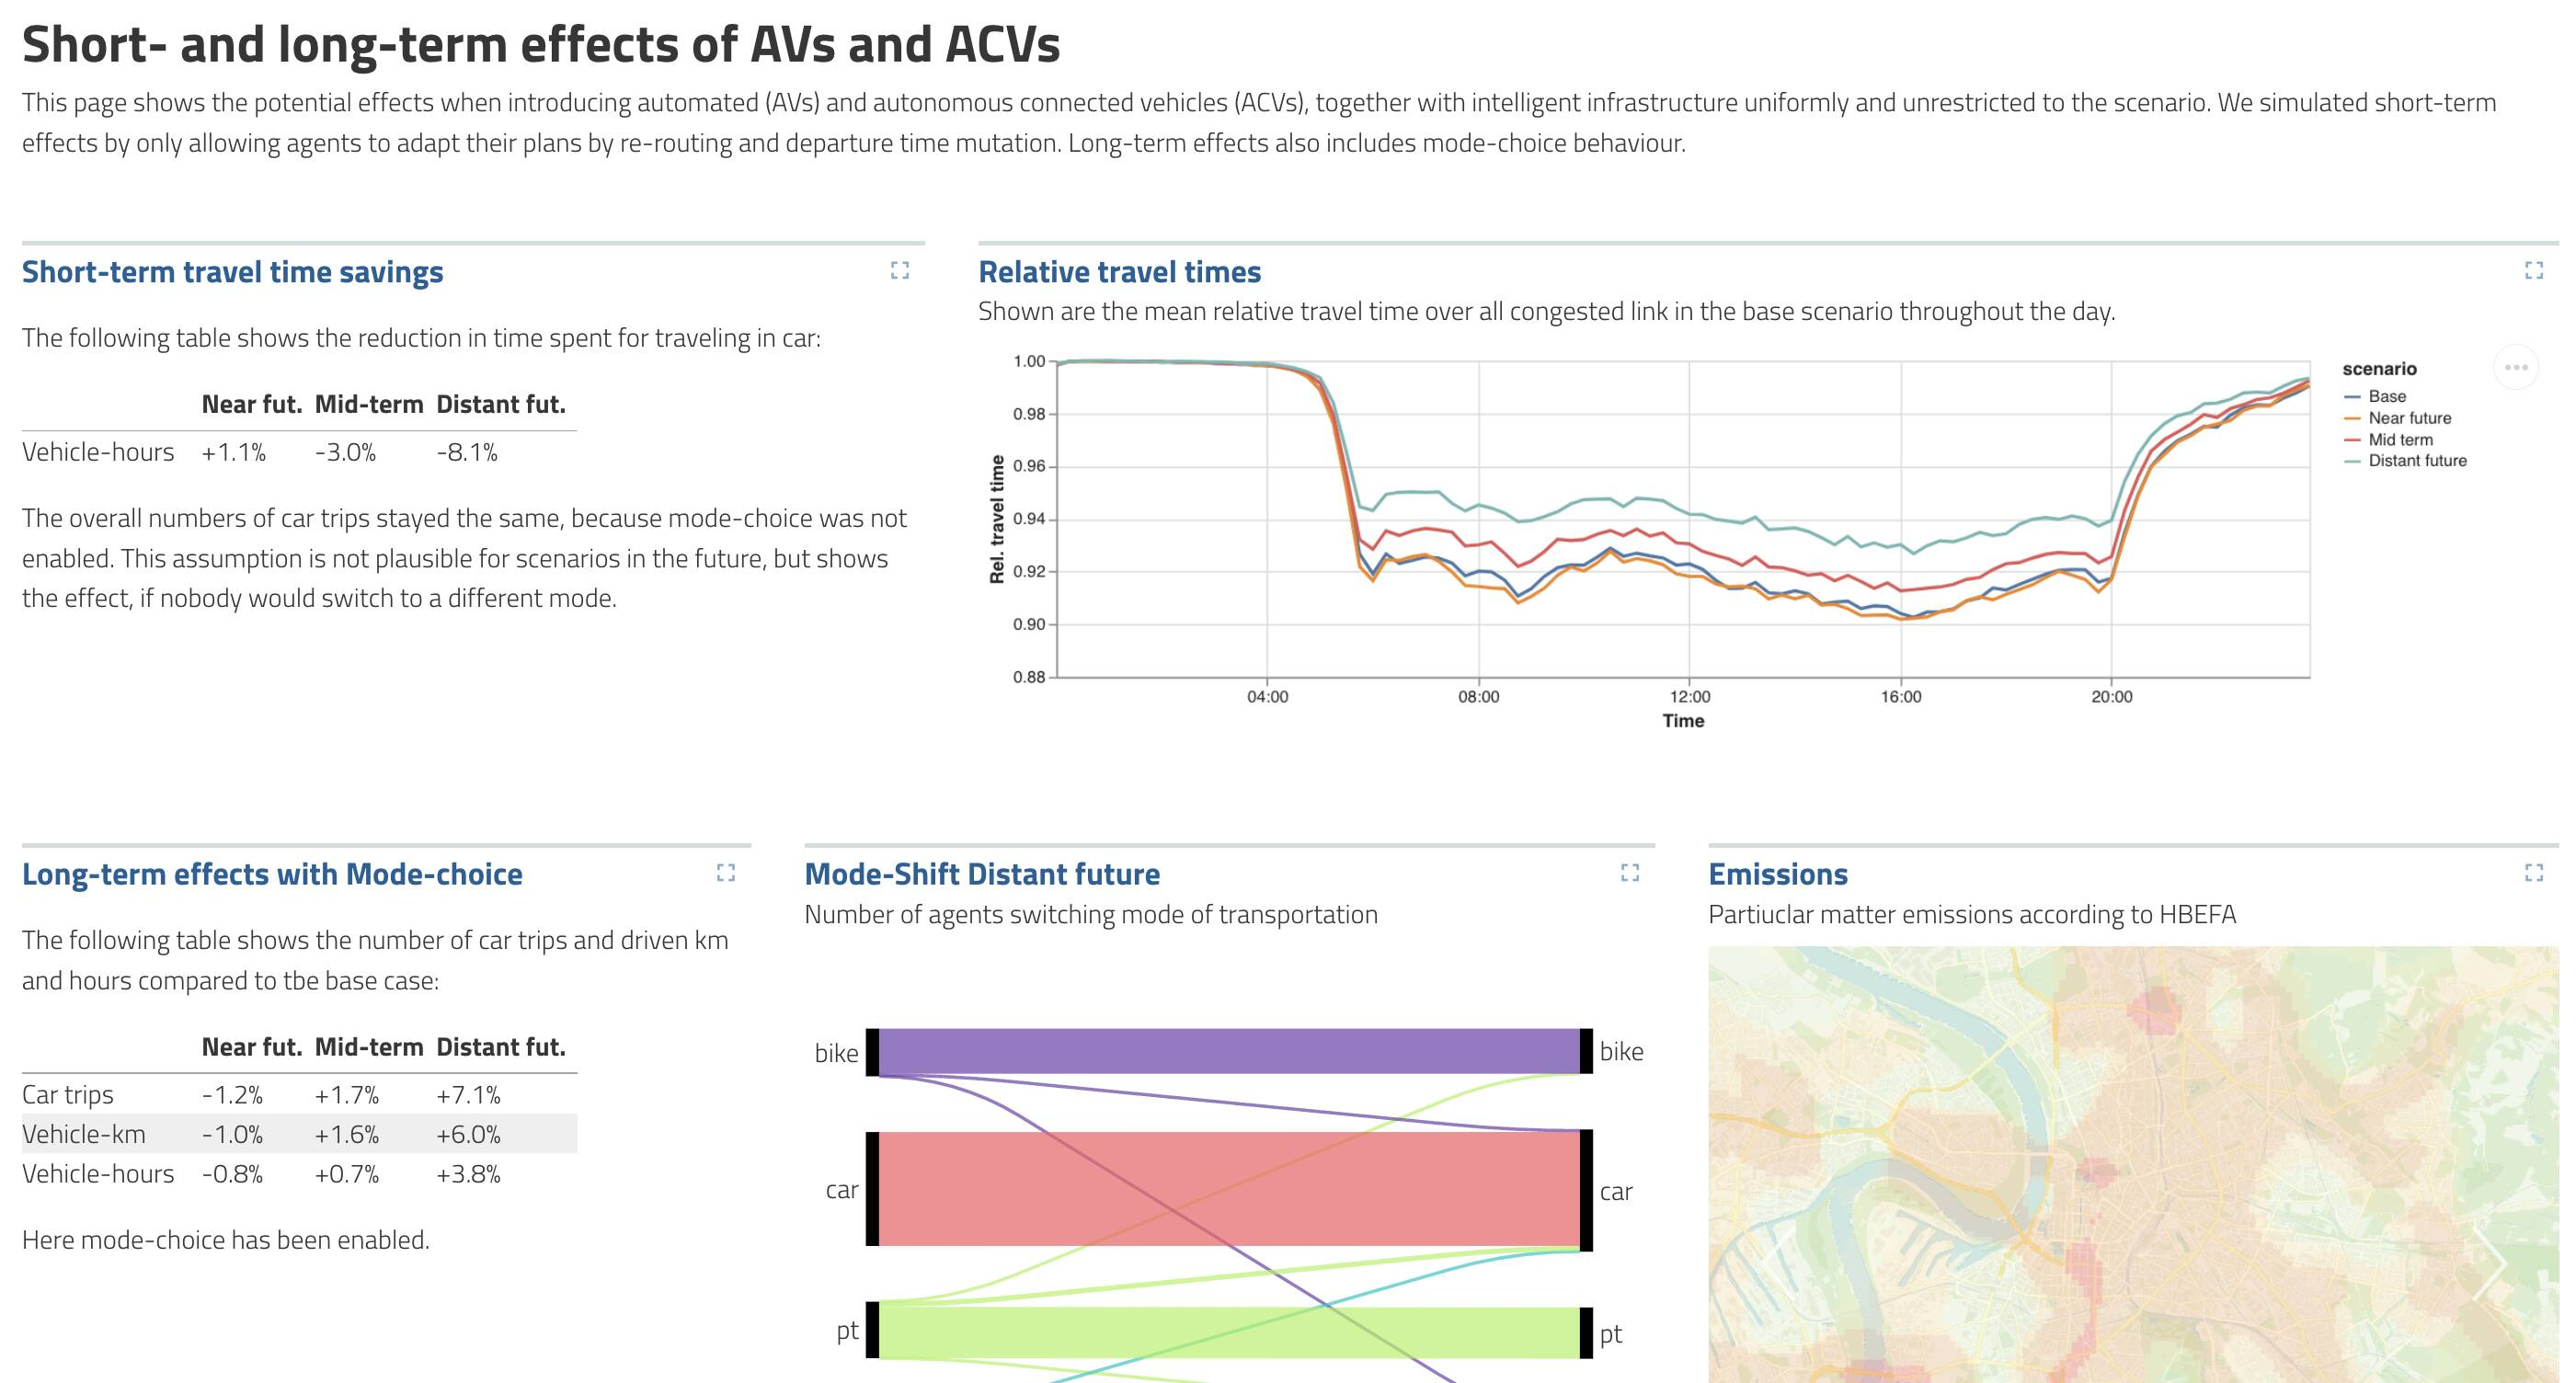
\includegraphics[width=\textwidth,height=3.2in]{images/fig-komod-next.jpg}
  \caption{KoMo:Dnext project dashboard}
  \label{fig:chart3}
\end{figure}


%% ======================================================================
%% ======================================================================
%% ======================================================================
\section{Discussion and Conclusions}

SimWrapper is under continuous development, and therefore its feature set is fluid. As of this writing, most of the basic needs of a transport planner are met: statistical summaries, area maps, network link displays, point data, and agent animations can all be displayed in cohesive dashboards. These are repeatable for comparison across scenarios, and publishable online. The technology has gone far beyond the old days of PDF reports.

The unique combination of features enables analysts to rapidly prototype and then publish their work, without requiring any programming. Feedback from initial users identifies many specific "pain points" in the use of the system: (1) initial onboarding is too complex, and a basic off-the-shelf dashboard would help create a starting point for new users; (2) documentation is extensive but always lagging behind current features; (3) YAML configuration files are flexible but difficult to master; and (4) a more consistent way to handle scenario comparisons is needed. Despite these issues, current users convey a very optimistic outlook on their continued use of SimWrapper.

These issues and some new visualizations are currently being considered for the continued development of the platform. Beyond the featureset of SimWrapper itself, longer-term questions remain about the viability of a small open-source research project in the face of commercial tools specifically designed to work with MATSim outputs, as well as very well-established and feature-rich open source tools such as GIS systems. There does appear to be a niche for a completely open source web platform which is specifically designed for transport microsimulation visualization.

Having confirmed the utility and capabilities of a fully browser-based data visualization platform for several projects at multiple agencies, SimWrapper is a viable visualization framework for transport planners interested in an open source tool for analyzing and publishing their work.

\section{Online resources}

SimWrapper main website: \url{https://vsp.berlin/simwrapper}

Companion tool for browsing local files: \url{https://pypi.org/project/simwrapper}


% \begin{figure}
%   \centering
% 	\begin{minipage}{.75\textwidth}
% 		\includegraphics[width=\textwidth]{chapters/06-simwrapper/images/charts.png.pdf}
% 		\caption{CHart: stuff.}
% 		\label{fig:chartychart}
% 	\end{minipage}
% \end{figure}


% \subsection{ Construction of references}
%
% References must be listed at the end of the paper. Do not begin them on a new page unless this is absolutely necessary. Authors should ensure that every reference in the text appears in the list of references and vice versa. Indicate references by \cite{Massimo2011} or \cite{Massimo2012} or \cite{Thomas2015} in the text.


% \subsection{File naming and delivery}
% Please title your files in this order `procedia acronym\_conference acronym\_authorslastname'.  Submit both the source file and the PDF to the Guest Editor.
%
% Artwork filenames should comply with the syntax ``aabbbbbb.ccc'', where:
% \begin{itemize}
% \item a = artwork component type
% \item b = manuscript reference code
% \item c = standard file extension
%
% Component types:
% \item gr = figure
% \item pl = plate
% \item sc = scheme
% \item fx = fixed graphic
% \end{itemize}


% \subsection{Footnotes}
% Footnotes should be avoided if possible. Necessary footnotes should be denoted in the text by consecutive superscript letters\footnote{Footnote text.}. The footnotes should be typed single spaced, and in smaller type size (8 pt), at the foot of the page in which they are mentioned, and separated from the main text by a one line space extending at the foot of the column. The `Els-footnote' style is available in the ``TeX Template'' for the text of the footnote.

% Please do not change the margins of the template as this can result in the footnote falling outside printing range.

% \begin{figure}[t]\vspace*{4pt}
% %\centerline{\includegraphics{fx1}\hspace*{5mm}\includegraphics{fx1}}
% \centerline{
\includegraphics{gr1}}
% \caption{(a) first picture; (b) second picture.}
% \end{figure}


\section{Acknowledgements}

This research was funded in part by the German Federal Ministry of Transport and Digital Infrastructure (funding number 16AVF2160). The author is thankful for the funding and support provided by the ActivitySim project. Some projects described in this paper use data provided by Senozon Deutschland GmbH.

\bibliography{paper}
\bibliographystyle{../src/elsarticle-harv}

\end{document}


%%
%% End of file `procs-template.tex'.
